\documentclass[11pt, a4paper]{article}
\usepackage[utf8]{inputenc}
\usepackage[T1]{fontenc}
\usepackage[french]{babel}
\usepackage[margin=1.8cm, top=2.2cm, bottom=2.2cm]{geometry}
\usepackage{amsmath, amssymb}
\usepackage{xcolor}
\usepackage{titlesec}
\usepackage{enumitem}
\usepackage{booktabs}
\usepackage{tabularx}
\usepackage{array}
\usepackage{listings}
\usepackage{tcolorbox}
\tcbuselibrary{skins,breakable}
\usepackage{tikz}
\usetikzlibrary{shapes,arrows.meta,positioning,calc}
\usepackage{fancyhdr}
\usepackage{graphicx}
\usepackage{hyperref}

% Palette de couleurs professionnelle
\definecolor{myblue}{RGB}{28, 85, 148}
\definecolor{myteal}{RGB}{0, 128, 128}
\definecolor{darkblue}{RGB}{15, 34, 64}
\definecolor{softblue}{RGB}{240, 245, 252}
\definecolor{softgreen}{RGB}{242, 249, 244}
\definecolor{softyellow}{RGB}{254, 250, 235}
\definecolor{borderblue}{RGB}{180, 205, 235}
\definecolor{codegray}{RGB}{245, 247, 250}
\definecolor{textgray}{RGB}{80, 80, 80}

\hypersetup{
    colorlinks=true,
    linkcolor=myblue,
    urlcolor=myteal,
    citecolor=myblue
}

% En-tête et pied de page
\pagestyle{fancy}
\fancyhf{}
\rhead{\small\textcolor{textgray}{Modélisation Dimensionnelle \& Data Warehouse}}
\lhead{\small\textcolor{myblue}{\textbf{Système Décisionnel Hospitalier}}}
\rfoot{\small Page \thepage}
\lfoot{\small\textcolor{textgray}{Support Pédagogique \& Correction Détaillée}}
\renewcommand{\headrulewidth}{0.4pt}
\renewcommand{\footrulewidth}{0.4pt}

% Format des titres
\titleformat{\section}
  {\normalfont\Large\bfseries\color{darkblue}}{\thesection}{1em}{}[{\titlerule[1pt]}]
\titleformat{\subsection}
  {\normalfont\large\bfseries\color{myblue}}{\thesubsection}{1em}{}
\titleformat{\subsubsection}
  {\normalfont\normalsize\bfseries\color{myteal}}{\thesubsubsection}{1em}{}

% Boîtes d'information élégantes
\newtcolorbox{infobox}[1]{
  colback=softblue,
  colframe=myblue,
  coltitle=white,
  fonttitle=\bfseries,
  title=#1,
  arc=2mm,
  boxrule=0.8pt,
  breakable
}

\newtcolorbox{methodobox}[1]{
  colback=softgreen,
  colframe=myteal,
  coltitle=white,
  fonttitle=\bfseries,
  title=#1,
  arc=2mm,
  boxrule=0.8pt,
  breakable
}

\newtcolorbox{alertbox}[1]{
  colback=softyellow,
  colframe=orange!80!black,
  coltitle=white,
  fonttitle=\bfseries,
  title=#1,
  arc=2mm,
  boxrule=0.8pt,
  breakable
}

% Configuration des listings SQL
\lstset{
  language=SQL,
  basicstyle=\ttfamily\footnotesize,
  backgroundcolor=\color{codegray},
  keywordstyle=\bfseries\color{myblue},
  commentstyle=\itshape\color{gray},
  stringstyle=\color{myteal},
  numbers=left,
  numberstyle=\tiny\color{textgray},
  stepnumber=1,
  numbersep=8pt,
  showstringspaces=false,
  breaklines=true,
  frame=single,
  rulecolor=\color{borderblue},
  tabsize=2,
  captionpos=b
}

\begin{document}

% ==============================================================================
% PAGE DE TITRE / BANDEAU D'EN-TÊTE
% ==============================================================================
\begin{center}
    {\large\textcolor{myteal}{\textbf{THÈME : PILOTAGE STRATÉGIQUE DE L'ACTIVITÉ MÉDICALE}}} \\
    \vspace{0.2cm}
    {\small\textcolor{textgray}{\textbf{Durée : 02H00 | Séance de Modélisation Conceptuelle \& Décisionnelle}}} \\
    \vspace{0.4cm}
    {\LARGE\textbf{\textcolor{darkblue}{Étude de Cas : Modernisation du Système Hospitalier}}} \\
    \vspace{0.2cm}
    {\large\textcolor{myblue}{\textit{Énoncé, Correction Exhaustive \& Guide d'Apprentissage Méthodologique}}}
    \vspace{0.3cm}
\end{center}
\hrule height 1.5pt \textcolor{darkblue}{}
\vspace{0.4cm}

% ==============================================================================
% SECTION 1 : ÉNONCÉ OFFICIEL DE L'ÉTUDE DE CAS
% ==============================================================================
\section{Énoncé de l'Étude de Cas}

\noindent\textbf{\textcolor{myblue}{Contexte général :}} \\
La direction d'un centre hospitalier de Rabat souhaite migrer vers un système de pilotage décisionnel pour optimiser sa gestion. Actuellement, le système transactionnel se contente d'enregistrer chaque interaction entre le corps médical et les usagers.

\vspace{0.2cm}
\noindent\textbf{\textcolor{myblue}{Récit du fonctionnement opérationnel :}} \\
Lorsqu'une visite est effectuée, le praticien renseigne une fiche comportant l'instant précis de l'acte, la durée effective de l'intervention ainsi que les frais de consultation facturés. Pour enrichir l'analyse, la direction souhaite croiser ces données avec le profil des patients (notamment leur âge au moment du soin, leur genre et leur provenance géographique) et l'expertise des intervenants (spécialité médicale et ancienneté dans la fonction). L'enjeu est de transformer cette masse d'informations brutes en leviers d'optimisation pour les ressources humaines et la prise en charge médicale.

\vspace{0.3cm}
\begin{infobox}{Travail à Faire (Exercice 1 : Analyse des Besoins et Extraction)}
En vous basant rigoureusement sur le récit de l'étude de cas :
\begin{enumerate}[label=\textbf{\arabic*.}]
    \item Identifier le \textbf{Processus Métier} fondamental à modéliser.
    \item Extraire du texte les \textbf{Indicateurs de Performance} (Mesures) nécessaires.
    \item Identifier les \textbf{Axes d'Analyse} (Dimensions) permettant de contextualiser ces mesures.
    \item Formuler quatre \textbf{questions d'analyse} critiques auxquelles le modèle devra répondre pour satisfaire les attentes de la direction.
\end{enumerate}
\end{infobox}

\vspace{0.2cm}
\begin{methodobox}{Rappel Méthodologique : Conception Dimensionnelle en 4 Étapes (Ralph Kimball)}
Pour structurer votre modélisation, appuyez-vous toujours sur la démarche canonique de Ralph Kimball :
\begin{itemize}[label=\textbullet]
    \item \textbf{Étape 1 : Sélectionner le Processus Métier.} Identifier l'événement opérationnel fondamental générateur de données (ex: la visite ou consultation médicale).
    \item \textbf{Étape 2 : Déclarer le Grain.} Déterminer le niveau de granularité le plus fin stocké dans la table de faits (ex: une ligne par acte médical dispensé).
    \item \textbf{Étape 3 : Choisir les Dimensions.} Répondre aux questions contextuelles : \textit{Qui ? Quand ? Où ? Quoi ?} (Temps, Patient, Praticien).
    \item \textbf{Étape 4 : Identifier les Faits.} Fixer les indicateurs numériques mesurables (durée d'intervention, montant facturé).
\end{itemize}
\end{methodobox}

\newpage

% ==============================================================================
% SECTION 2 : CORRECTION COMPLÈTE ET DÉTAILLÉE
% ==============================================================================
\section{Correction Détaillée de l'Étude de Cas}

\subsection{1. Identification du Processus Métier}
\begin{itemize}[label=$\blacktriangleright$]
    \item \textbf{Processus retenu :} \textbf{L'activité des consultations et actes médicaux} (ou \textit{la réalisation d'un acte de soin lors d'une visite}).
    \item \textbf{Justification décisionnelle :} Dans le système opérationnel de l'hôpital, l'événement clé qui consomme du temps soignant, engage des ressources matérielles et génère une facturation est l'interaction de consultation. C'est le flux d'activité à piloter pour optimiser les plannings RH et l'efficacité des soins.
\end{itemize}

\subsection{2. Déclaration du Grain (Niveau de Finesse Atomique)}
\begin{itemize}[label=$\blacktriangleright$]
    \item \textbf{Grain retenu :} \textbf{Une ligne par visite médicale / acte médical réalisé pour un patient donné par un praticien à un instant précis}.
    \item \textbf{Règle d'or de Kimball :} Toujours déclarer le grain le plus fin (grain atomique). Un grain atomique autorise toutes les agrégations postérieures possibles (sommes par mois, moyennes par service, comparaisons annuelles) sans jamais détruire d'information.
\end{itemize}

\subsection{3. Extraction des Indicateurs de Performance (Mesures / Faits)}
Les faits sont les grandeurs quantitatives mesurables rattachées à chaque occurrence de l'événement :

\begin{center}
\renewcommand{\arraystretch}{1.3}
\begin{tabularx}{\textwidth}{p{4.2cm} p{2.8cm} p{2.5cm} X}
\toprule
\textbf{Nom de la Mesure} & \textbf{Type de Donnée} & \textbf{Additivité} & \textbf{Rôle \& Intérêt Décisionnel} \\
\midrule
\texttt{duree\_intervention\_min} & Entier (Minutes) & Additive & Temps soignant effectif ; cumulable pour mesurer la charge globale de travail. \\
\texttt{frais\_consultation} & Numérique (MAD) & Additive & Montant facturé à l'usager ; cumulable pour le calcul du chiffre d'affaires. \\
\texttt{nb\_visites} & Entier (Fixé à 1) & Additive & Compteur technique unitaire facilitant les calculs de volumes (\texttt{SUM}). \\
\texttt{duree\_moyenne\_acte} & Décimal (Calculé) & Non-additive & Mesure dérivée : \texttt{SUM(duree) / SUM(nb\_visites)}. \\
\texttt{recette\_moyenne\_patient} & Décimal (Calculé) & Non-additive & Mesure dérivée : \texttt{SUM(frais) / COUNT(DISTINCT patient)}. \\
\bottomrule
\end{tabularx}
\end{center}

\subsection{4. Définition des Axes d'Analyse (Dimensions et Dictionnaires d'Attributs)}

\noindent Les dimensions apportent le contexte textuel et descriptif permettant de filtrer, regrouper et trancher les faits :

\begin{enumerate}[label=\textbf{\alph*.}]
    \item \textbf{Dimension Temps (\texttt{DIM\_TEMPS}) — Axe « Quand ? » :}
    \begin{itemize}
        \item \textbf{Clé primaire surrogate :} \texttt{date\_key} (entier au format \texttt{YYYYMMDD}, ex: \texttt{20261025}).
        \item \textbf{Attributs de calendrier :} \texttt{date\_complete}, \texttt{jour\_mois}, \texttt{nom\_jour}, \texttt{semaine}, \texttt{mois}, \texttt{nom\_mois}, \texttt{trimestre}, \texttt{annee}, \texttt{indicateur\_weekend}, \texttt{indicateur\_ferie}.
        \item \textbf{Attributs horaires :} \texttt{heure\_acte}, \texttt{tranche\_horaire} (ex: Matin [08h-12h], Après-midi [12h-18h], Nuit [18h-08h]).
    \end{itemize}

    \item \textbf{Dimension Patient (\texttt{DIM\_PATIENT}) — Axe « Pour qui ? » :}
    \begin{itemize}
        \item \textbf{Clé primaire surrogate :} \texttt{patient\_key} (entier séquentiel anonymisé).
        \item \textbf{Clé naturelle source :} \texttt{code\_patient\_source} (identifiant du dossier médical informatisé).
        \item \textbf{Attributs démographiques :} \texttt{genre} (H/F), \texttt{age\_au\_soin}, \texttt{tranche\_age} (ex: 0-17 pédiatrique, 18-35 jeune actif, 36-60 adulte, 60+ senior).
        \item \textbf{Attributs géographiques :} \texttt{ville\_provenance} (Rabat, Salé, Kénitra, etc.), \texttt{region}, \texttt{quartier}.
    \end{itemize}

    \item \textbf{Dimension Praticien (\texttt{DIM\_PRATICIEN}) — Axe « Par qui ? » :}
    \begin{itemize}
        \item \textbf{Clé primaire surrogate :} \texttt{praticien\_key} (entier séquentiel).
        \item \textbf{Clé naturelle source :} \texttt{matricule\_praticien}.
        \item \textbf{Attributs professionnels :} \texttt{nom\_praticien}, \texttt{specialite\_medicale} (Cardiologie, Médecine Générale, Neurologie...), \texttt{anciennete\_annees}, \texttt{tranche\_anciennete} (moins de 2 ans novice, 2-10 ans expérimenté, plus de 10 ans expert), \texttt{statut\_intervenant} (Interne, Résident, Titulaire, Chef de service).
    \end{itemize}
\end{enumerate}

\vspace{0.4cm}
\subsection{5. Modélisation Conceptuelle : Schéma en Étoile}

Le schéma en étoile structure l'entrepôt en positionnant la table de faits au centre, entourée de ses dimensions dénormalisées :

\begin{figure}[htbp]
\centering
\begin{tikzpicture}[
  node distance=1.5cm,
  fait/.style={rectangle, rounded corners=3pt, draw=myblue, fill=darkblue, text=white, minimum width=5.2cm, minimum height=3.4cm, align=center, font=\small},
  dim/.style={rectangle, rounded corners=3pt, draw=myteal, fill=myteal!10, minimum width=4.5cm, minimum height=2.5cm, align=left, font=\small},
  fleche/.style={-{Latex[length=3mm]}, thick, draw=myblue}
]

% Table de faits
\node[fait] (fact) at (0,0) {
  \textbf{\large FACT\_VISITES\_MEDICALES}\\[0.15cm]
  \par\vspace{2pt}\hrulefill\par\vspace{4pt}
  \textbf{\textit{Clés étrangères (FK) :}}\\
  $\bullet$ \texttt{date\_key} (FK $\rightarrow$ DIM\_TEMPS)\\
  $\bullet$ \texttt{patient\_key} (FK $\rightarrow$ DIM\_PATIENT)\\
  $\bullet$ \texttt{praticien\_key} (FK $\rightarrow$ DIM\_PRATICIEN)\\[0.15cm]
  \textbf{\textit{Mesures numériques :}}\\
  $\bullet$ \texttt{duree\_intervention\_min}\\
  $\bullet$ \texttt{frais\_consultation}\\
  $\bullet$ \texttt{nb\_visites} (= 1)
};

% Dimensions
\node[dim] (temps) at (-6.2, 3.2) {
  \textbf{\textcolor{myblue}{DIM\_TEMPS}}\\[0.1cm]
  \par\vspace{2pt}\hrulefill\par\vspace{4pt}
  \textbf{PK : \texttt{date\_key}}\\
  $\bullet$ \texttt{date\_complete}\\
  $\bullet$ \texttt{moment\_journee}\\
  $\bullet$ \texttt{mois / annee}\\
  $\bullet$ \texttt{est\_jour\_ferie}
};

\node[dim] (patient) at (6.2, 3.2) {
  \textbf{\textcolor{myblue}{DIM\_PATIENT}}\\[0.1cm]
  \par\vspace{2pt}\hrulefill\par\vspace{4pt}
  \textbf{PK : \texttt{patient\_key}}\\
  $\bullet$ \texttt{genre}\\
  $\bullet$ \texttt{age\_au\_soin}\\
  $\bullet$ \texttt{tranche\_age}\\
  $\bullet$ \texttt{ville\_provenance}
};

\node[dim] (praticien) at (0, -4.2) {
  \textbf{\textcolor{myblue}{DIM\_PRATICIEN}}\\[0.1cm]
  \par\vspace{2pt}\hrulefill\par\vspace{4pt}
  \textbf{PK : \texttt{praticien\_key}}\\
  $\bullet$ \texttt{nom\_praticien}\\
  $\bullet$ \texttt{specialite\_medicale}\\
  $\bullet$ \texttt{anciennete\_annees}\\
  $\bullet$ \texttt{tranche\_anciennete}
};

% Liaisons
\draw[fleche] (temps.south east) -- (fact.north west);
\draw[fleche] (patient.south west) -- (fact.north east);
\draw[fleche] (praticien.north) -- (fact.south);

\end{tikzpicture}
\caption{Schéma en Étoile du Système Hospitalier}
\end{figure}

\subsection{6. Implémentation SQL (Script DDL d'Alimentation du Schéma)}

\begin{lstlisting}[caption={Script SQL de création des tables dimensionnelles et de faits}]
-- 1. Dimension Temps
CREATE TABLE dim_temps (
    date_key          INTEGER PRIMARY KEY, -- Format YYYYMMDD
    date_complete     DATE NOT NULL,
    heure_acte        TIME NOT NULL,
    moment_journee    VARCHAR(20) NOT NULL, -- Matin, Apres-midi, Nuit
    jour_semaine      VARCHAR(15) NOT NULL,
    mois              INTEGER NOT NULL,
    nom_mois          VARCHAR(15) NOT NULL,
    trimestre         INTEGER NOT NULL,
    annee             INTEGER NOT NULL,
    est_jour_ferie    BOOLEAN DEFAULT FALSE
);

-- 2. Dimension Patient
CREATE TABLE dim_patient (
    patient_key       SERIAL PRIMARY KEY,  -- Cle surrogate
    code_patient_src  VARCHAR(50) NOT NULL,
    genre             CHAR(1) CHECK (genre IN ('M', 'F')),
    age_au_soin       INTEGER NOT NULL,
    tranche_age       VARCHAR(30) NOT NULL,
    ville_provenance  VARCHAR(100) NOT NULL,
    region            VARCHAR(100) NOT NULL
);

-- 3. Dimension Praticien
CREATE TABLE dim_praticien (
    praticien_key     SERIAL PRIMARY KEY,  -- Cle surrogate
    matricule_src     VARCHAR(50) NOT NULL,
    nom_praticien     VARCHAR(100) NOT NULL,
    specialite        VARCHAR(100) NOT NULL,
    anciennete_annees INTEGER NOT NULL,
    statut            VARCHAR(50) NOT NULL
);

-- 4. Table de Faits Centrale
CREATE TABLE fact_visites_medicales (
    visite_id              BIGSERIAL PRIMARY KEY,
    date_key               INTEGER NOT NULL REFERENCES dim_temps(date_key),
    patient_key            INTEGER NOT NULL REFERENCES dim_patient(patient_key),
    praticien_key          INTEGER NOT NULL REFERENCES dim_praticien(praticien_key),
    duree_intervention_min INTEGER NOT NULL CHECK (duree_intervention_min > 0),
    frais_consultation     NUMERIC(10,2) NOT NULL CHECK (frais_consultation >= 0),
    nb_visites             INTEGER DEFAULT 1
);
\end{lstlisting}

\newpage

\subsection{7. Formulation et Réponses aux 4 Questions d'Analyse Critiques}

\noindent\textbf{Question 1 (Gestion des RH \& Productivité) :} \\
\textit{« Quelle est la durée moyenne d'une consultation par spécialité médicale et selon la tranche d'ancienneté du praticien ? »}
\begin{itemize}[label=$\rightarrow$]
    \item \textbf{Objectif directionnel :} Évaluer si les praticiens juniors passent significativement plus de temps par acte que les seniors, identifier les spécialités sous tension horaire et dimensionner les recrutements.
    \item \textbf{Requête analytique cible :}
    \begin{lstlisting}
SELECT p.specialite, p.anciennete_annees,
       ROUND(AVG(f.duree_intervention_min), 1) AS duree_moyenne_min,
       COUNT(f.visite_id) AS total_consultations
FROM fact_visites_medicales f
JOIN dim_praticien p ON f.praticien_key = p.praticien_key
GROUP BY p.specialite, p.anciennete_annees
ORDER BY duree_moyenne_min DESC;
    \end{lstlisting}
\end{itemize}

\vspace{0.2cm}
\noindent\textbf{Question 2 (Rentabilité \& Économie de la Santé) :} \\
\textit{« Quel est le chiffre d'affaires mensuel généré par chaque spécialité et quelle est la répartition des recettes par moment de la journée (journée normale vs garde de nuit) ? »}
\begin{itemize}[label=$\rightarrow$]
    \item \textbf{Objectif directionnel :} Ajuster la grille tarifaire, évaluer la rentabilité relative des services et calibrer les primes des gardes de nuit.
    \item \textbf{Requête analytique cible :}
    \begin{lstlisting}
SELECT t.annee, t.nom_mois, p.specialite, t.moment_journee,
       SUM(f.frais_consultation) AS chiffre_affaires_total,
       ROUND(AVG(f.frais_consultation), 2) AS tarif_moyen_facture
FROM fact_visites_medicales f
JOIN dim_temps t ON f.date_key = t.date_key
JOIN dim_praticien p ON f.praticien_key = p.praticien_key
GROUP BY t.annee, t.nom_mois, p.specialite, t.moment_journee;
    \end{lstlisting}
\end{itemize}

\vspace{0.2cm}
\noindent\textbf{Question 3 (Couverture Territoriale \& Épidémiologie) :} \\
\textit{« Quelle est la provenance géographique des patients selon leur tranche d'âge et les pathologies/spécialités consultées ? »}
\begin{itemize}[label=$\rightarrow$]
    \item \textbf{Objectif directionnel :} Déterminer si certains bassins de population (villes voisines) se déplacent spécifiquement pour des spécialités rares, et planifier l'ouverture éventuelle d'annexes médicales.
    \item \textbf{Requête analytique cible :}
    \begin{lstlisting}
SELECT pa.ville_provenance, pa.tranche_age, pr.specialite,
       COUNT(f.visite_id) AS volume_patients
FROM fact_visites_medicales f
JOIN dim_patient pa ON f.patient_key = pa.patient_key
JOIN dim_praticien pr ON f.praticien_key = pr.praticien_key
GROUP BY pa.ville_provenance, pa.tranche_age, pr.specialite
ORDER BY volume_patients DESC;
    \end{lstlisting}
\end{itemize}

\vspace{0.2cm}
\noindent\textbf{Question 4 (Saisonnalité \& Saturation Temporelle) :} \\
\textit{« Quels sont les jours de la semaine et les mois présentant une sur-sollicitation critique en nombre de consultations pour les tranches d'âge vulnérables (enfants et seniors) ? »}
\begin{itemize}[label=$\rightarrow$]
    \item \textbf{Objectif directionnel :} Anticiper les épidémies saisonnières (ex: grippe hivernale chez les seniors, bronchiolites pédiatriques) pour planifier les congés du personnel et renforcer les astreintes.
\end{itemize}

\newpage

% ==============================================================================
% SECTION 3 : SYNTHÈSE THÉORIQUE DU COURS & CONCEPTS CLÉS
% ==============================================================================
\section{Concepts Fondamentaux \& Synthèse du Cours}

\subsection{1. La Dichotomie OLTP vs OLAP}
La première compétence d'un ingénieur de données est de distinguer formellement la production transactionnelle de l'exploitation analytique :

\begin{center}
\renewcommand{\arraystretch}{1.25}
\begin{tabularx}{\textwidth}{p{3.5cm} X X}
\toprule
\textbf{Critère de Comparaison} & \textbf{OLTP (\textit{Run the Business})} & \textbf{OLAP (\textit{Steer the Business})} \\
\midrule
\textbf{Finalité} & Exécuter les opérations quotidiennes de l'organisation en temps réel. & Guider les décisions stratégiques et tactiques de la direction. \\
\textbf{Modélisation} & Fortement normalisée (3NF, réduction des redondances). & Dénormalisée (schémas en étoile ou en flocon). \\
\textbf{Opérations dominantes} & Écritures rapides et ciblées (\texttt{INSERT}, \texttt{UPDATE}). & Lectures massives et agrégations (\texttt{SUM}, \texttt{AVG}). \\
\textbf{Garanties requises} & Propriétés ACID strictes (Atomicité, Cohérence, Isolation, Durabilité). & Rapidité de balayage et performances d'agrégation. \\
\textbf{Historique conservé} & État courant (les mises à jour écrasent l'état antérieur). & Historique sur plusieurs années (non volatil, horodaté). \\
\textbf{Pourquoi séparer ?} & \multicolumn{2}{p{12cm}}{\textbf{Prévention de la contention :} Une requête analytique qui balaye 5 ans de données monopolise le CPU, sature la mémoire vive et pose des verrous partagés (\textit{S-Locks}), bloquant ainsi les transactions d'écriture opérationnelles (\textit{X-Locks}).} \\
\bottomrule
\end{tabularx}
\end{center}

\subsection{2. Les 4 Piliers d'Inmon Définissant un Data Warehouse}
Un entrepôt de données se caractérise obligatoirement par les quatre propriétés formalisées par Bill Inmon :
\begin{enumerate}
    \item \textbf{Orienté Sujet (\textit{Subject-Oriented}) :} Il organise les données par thématique métier (Ventes, Soins, Patients) plutôt que par application informatique source.
    \item \textbf{Intégré (\textit{Integrated}) :} Il résout les hétérogénéités syntaxiques et sémantiques entre sources différentes (harmonisation des formats de dates, des unités de mesure et des codes de référence).
    \item \textbf{Non-Volatil (\textit{Non-Volatile}) :} Les données y sont immuables. On ne pratique aucun effacement ni écrasement en production pour préserver l'intégrité de la mémoire historique.
    \item \textbf{Historisé / Orienté dans le temps (\textit{Time-Variant}) :} Chaque enregistrement est explicitement lié à un repère temporel pour analyser les évolutions et tendances.
\end{enumerate}

\subsection{3. Architecture en 5 Couches \& Architecture Médaillon}

\begin{figure}[htbp]
\centering
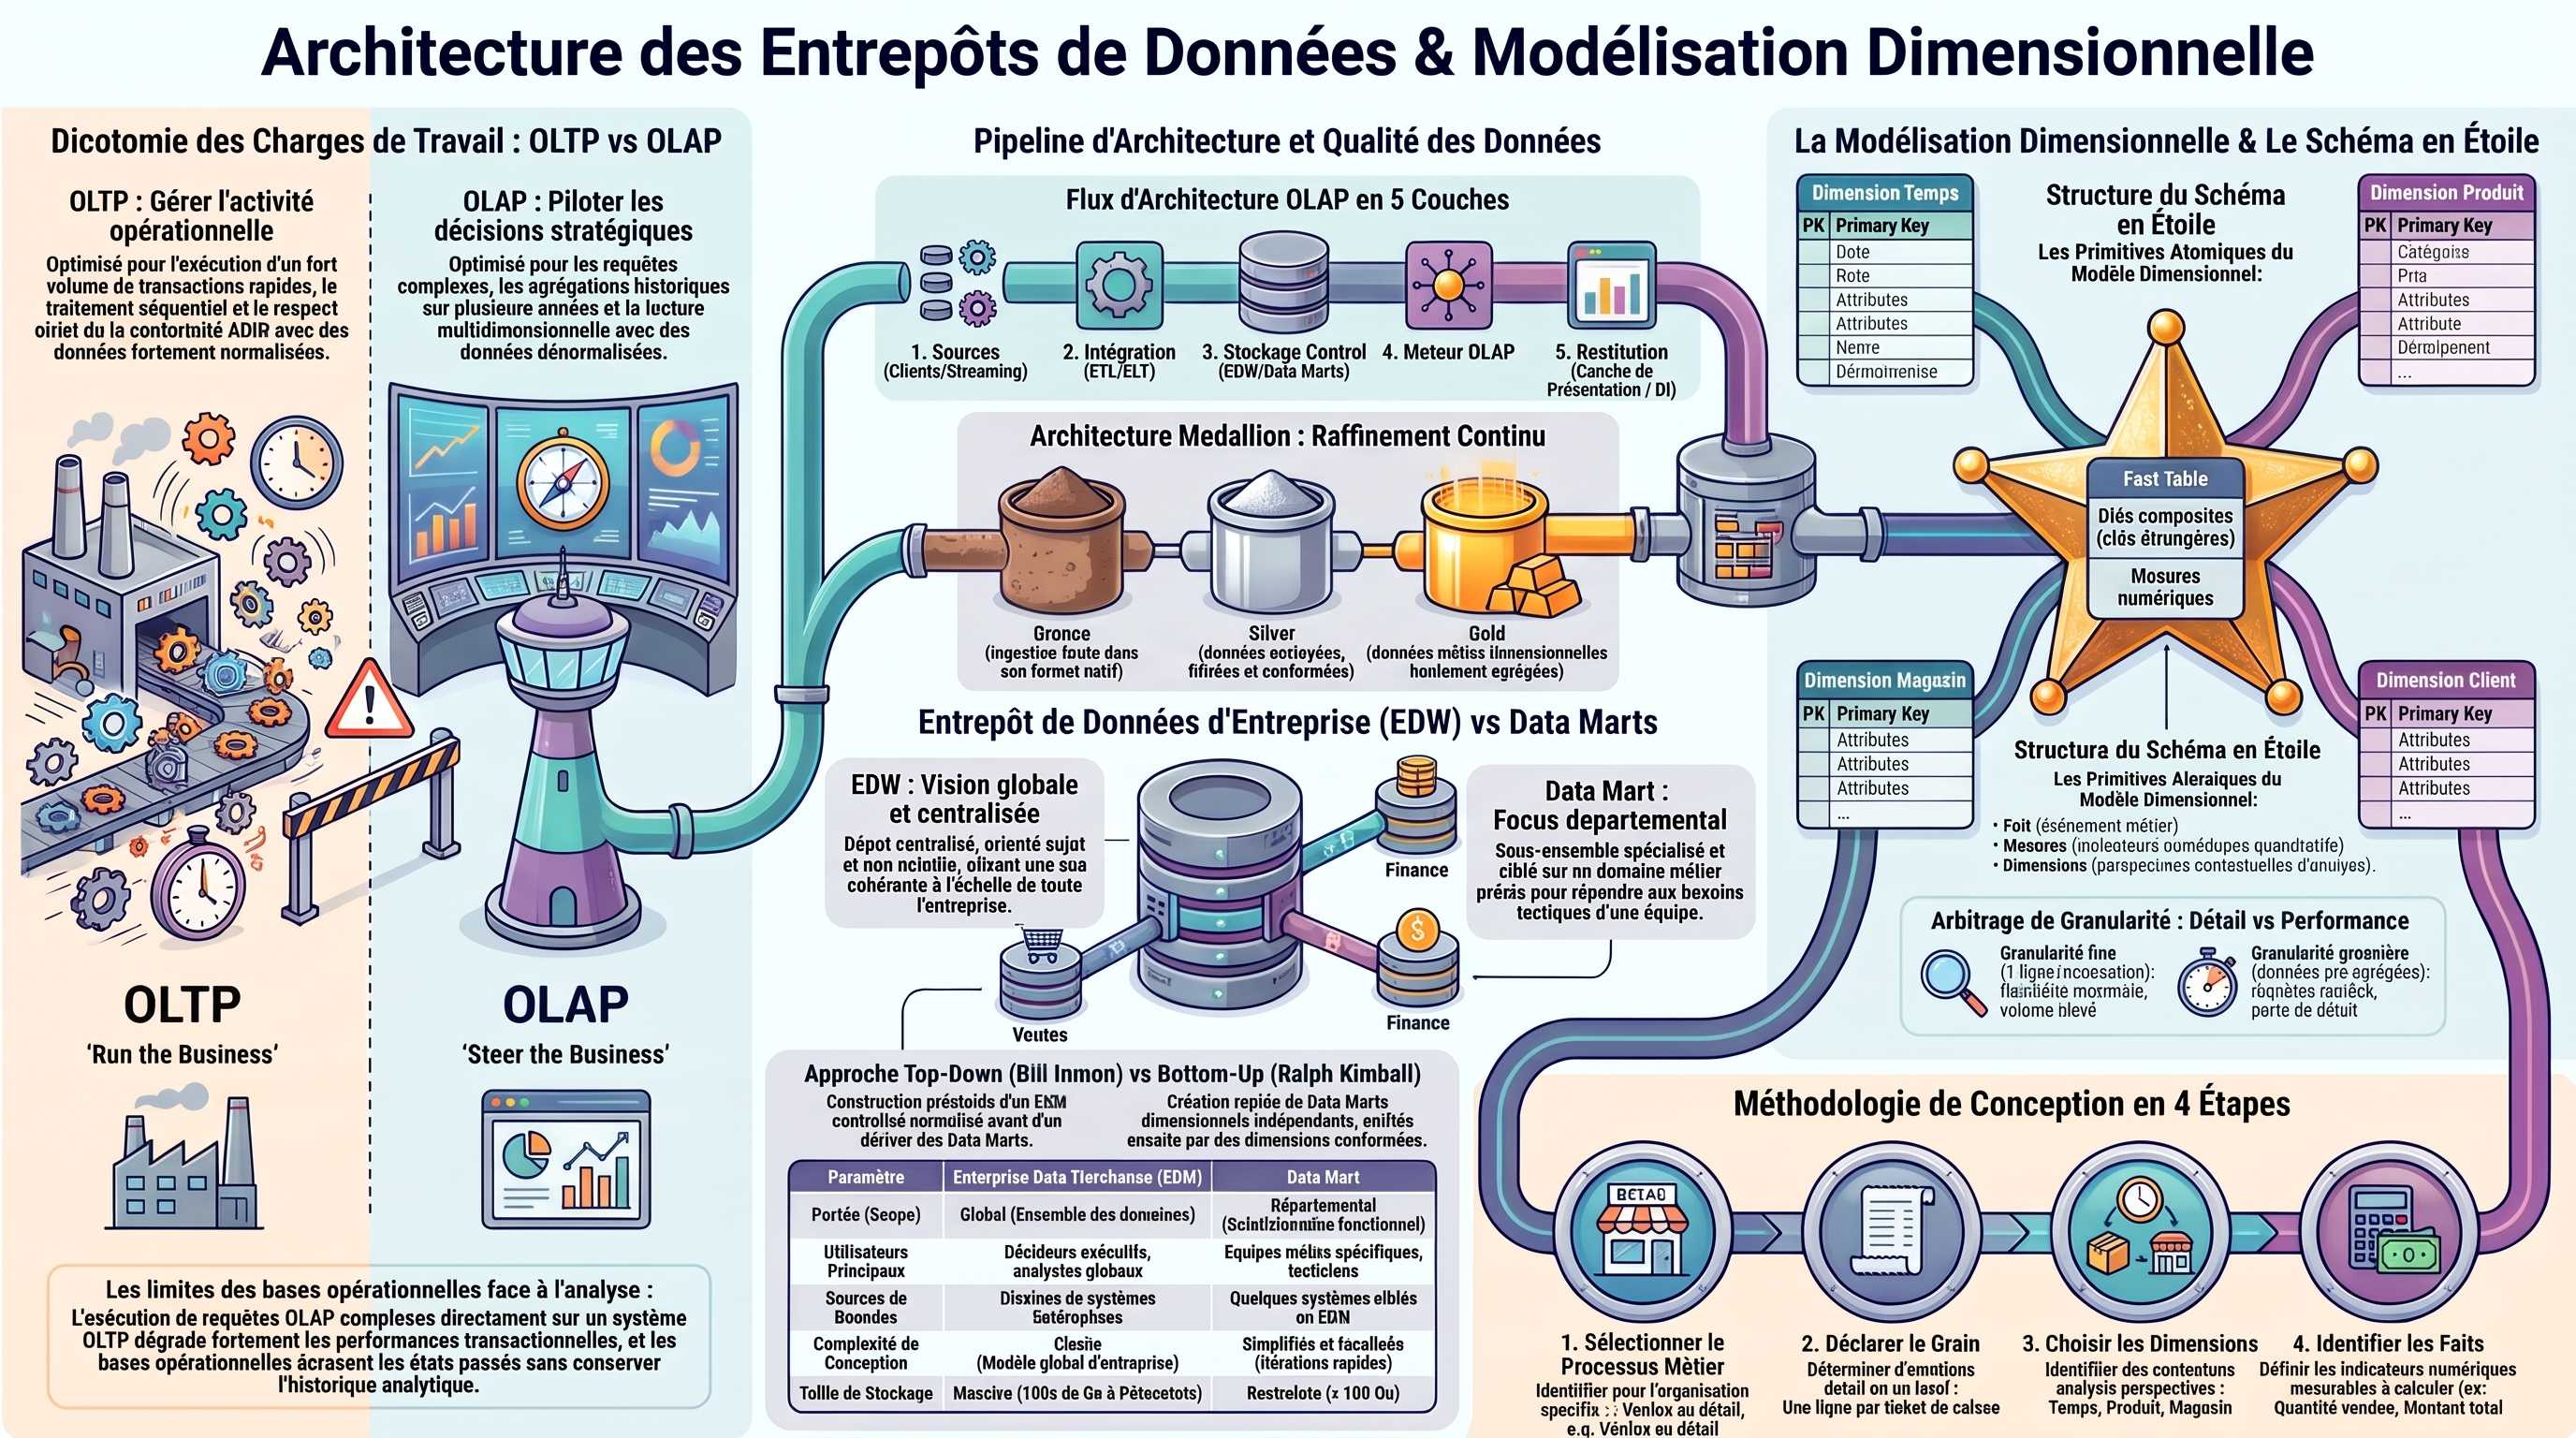
\includegraphics[width=\textwidth, height=0.7\textheight, keepaspectratio]{architecture_entrepot_donnees.png}
\caption{Architecture globale des entrepôts de données et modélisation dimensionnelle}
\end{figure}

\noindent\textbf{Le flux en 5 couches :}
\begin{enumerate}[label=\textbf{\arabic*.}]
    \item \textbf{Sources de données :} Systèmes transactionnels (ERP, CRM, SI Hospitalier), fichiers plats, flux IoT/Streaming.
    \item \textbf{Services d'intégration (ETL / ELT) :} Extraction des données sources, nettoyage, standardisation et chargement.
    \item \textbf{Stockage Central (EDW / Data Marts) :} Référentiel consolidé central et magasins spécialisés par département.
    \item \textbf{Moteur OLAP :} Moteurs d'indexation colonne et de calcul multidimensionnel optimisés pour les requêtes décisionnelles.
    \item \textbf{Couche de Restitution :} Tableaux de bord de Business Intelligence (PowerBI, Tableau), reporting réglementaire et Data Mining.
\end{enumerate}

\vspace{0.2cm}
\noindent\textbf{Le raffinement continu de l'Architecture Médaillon :}
\begin{itemize}
    \item \textbf{Bronze (Atterrissage Brut) :} Stockage des flux sources dans leur format brut natif (\textit{raw ingestion}).
    \item \textbf{Silver (Conformé \& Nettoyé) :} Données dédoublonnées, filtrées, typées et conformées aux règles d'entreprise.
    \item \textbf{Gold (Agrégé \& Modélisé) :} Schémas en étoile finaux directement interrogeables par les outils BI et les data scientists.
\end{itemize}

\newpage

\subsection{4. Duel d'Écoles : Bill Inmon vs Ralph Kimball}

\begin{figure}[htbp]
\centering
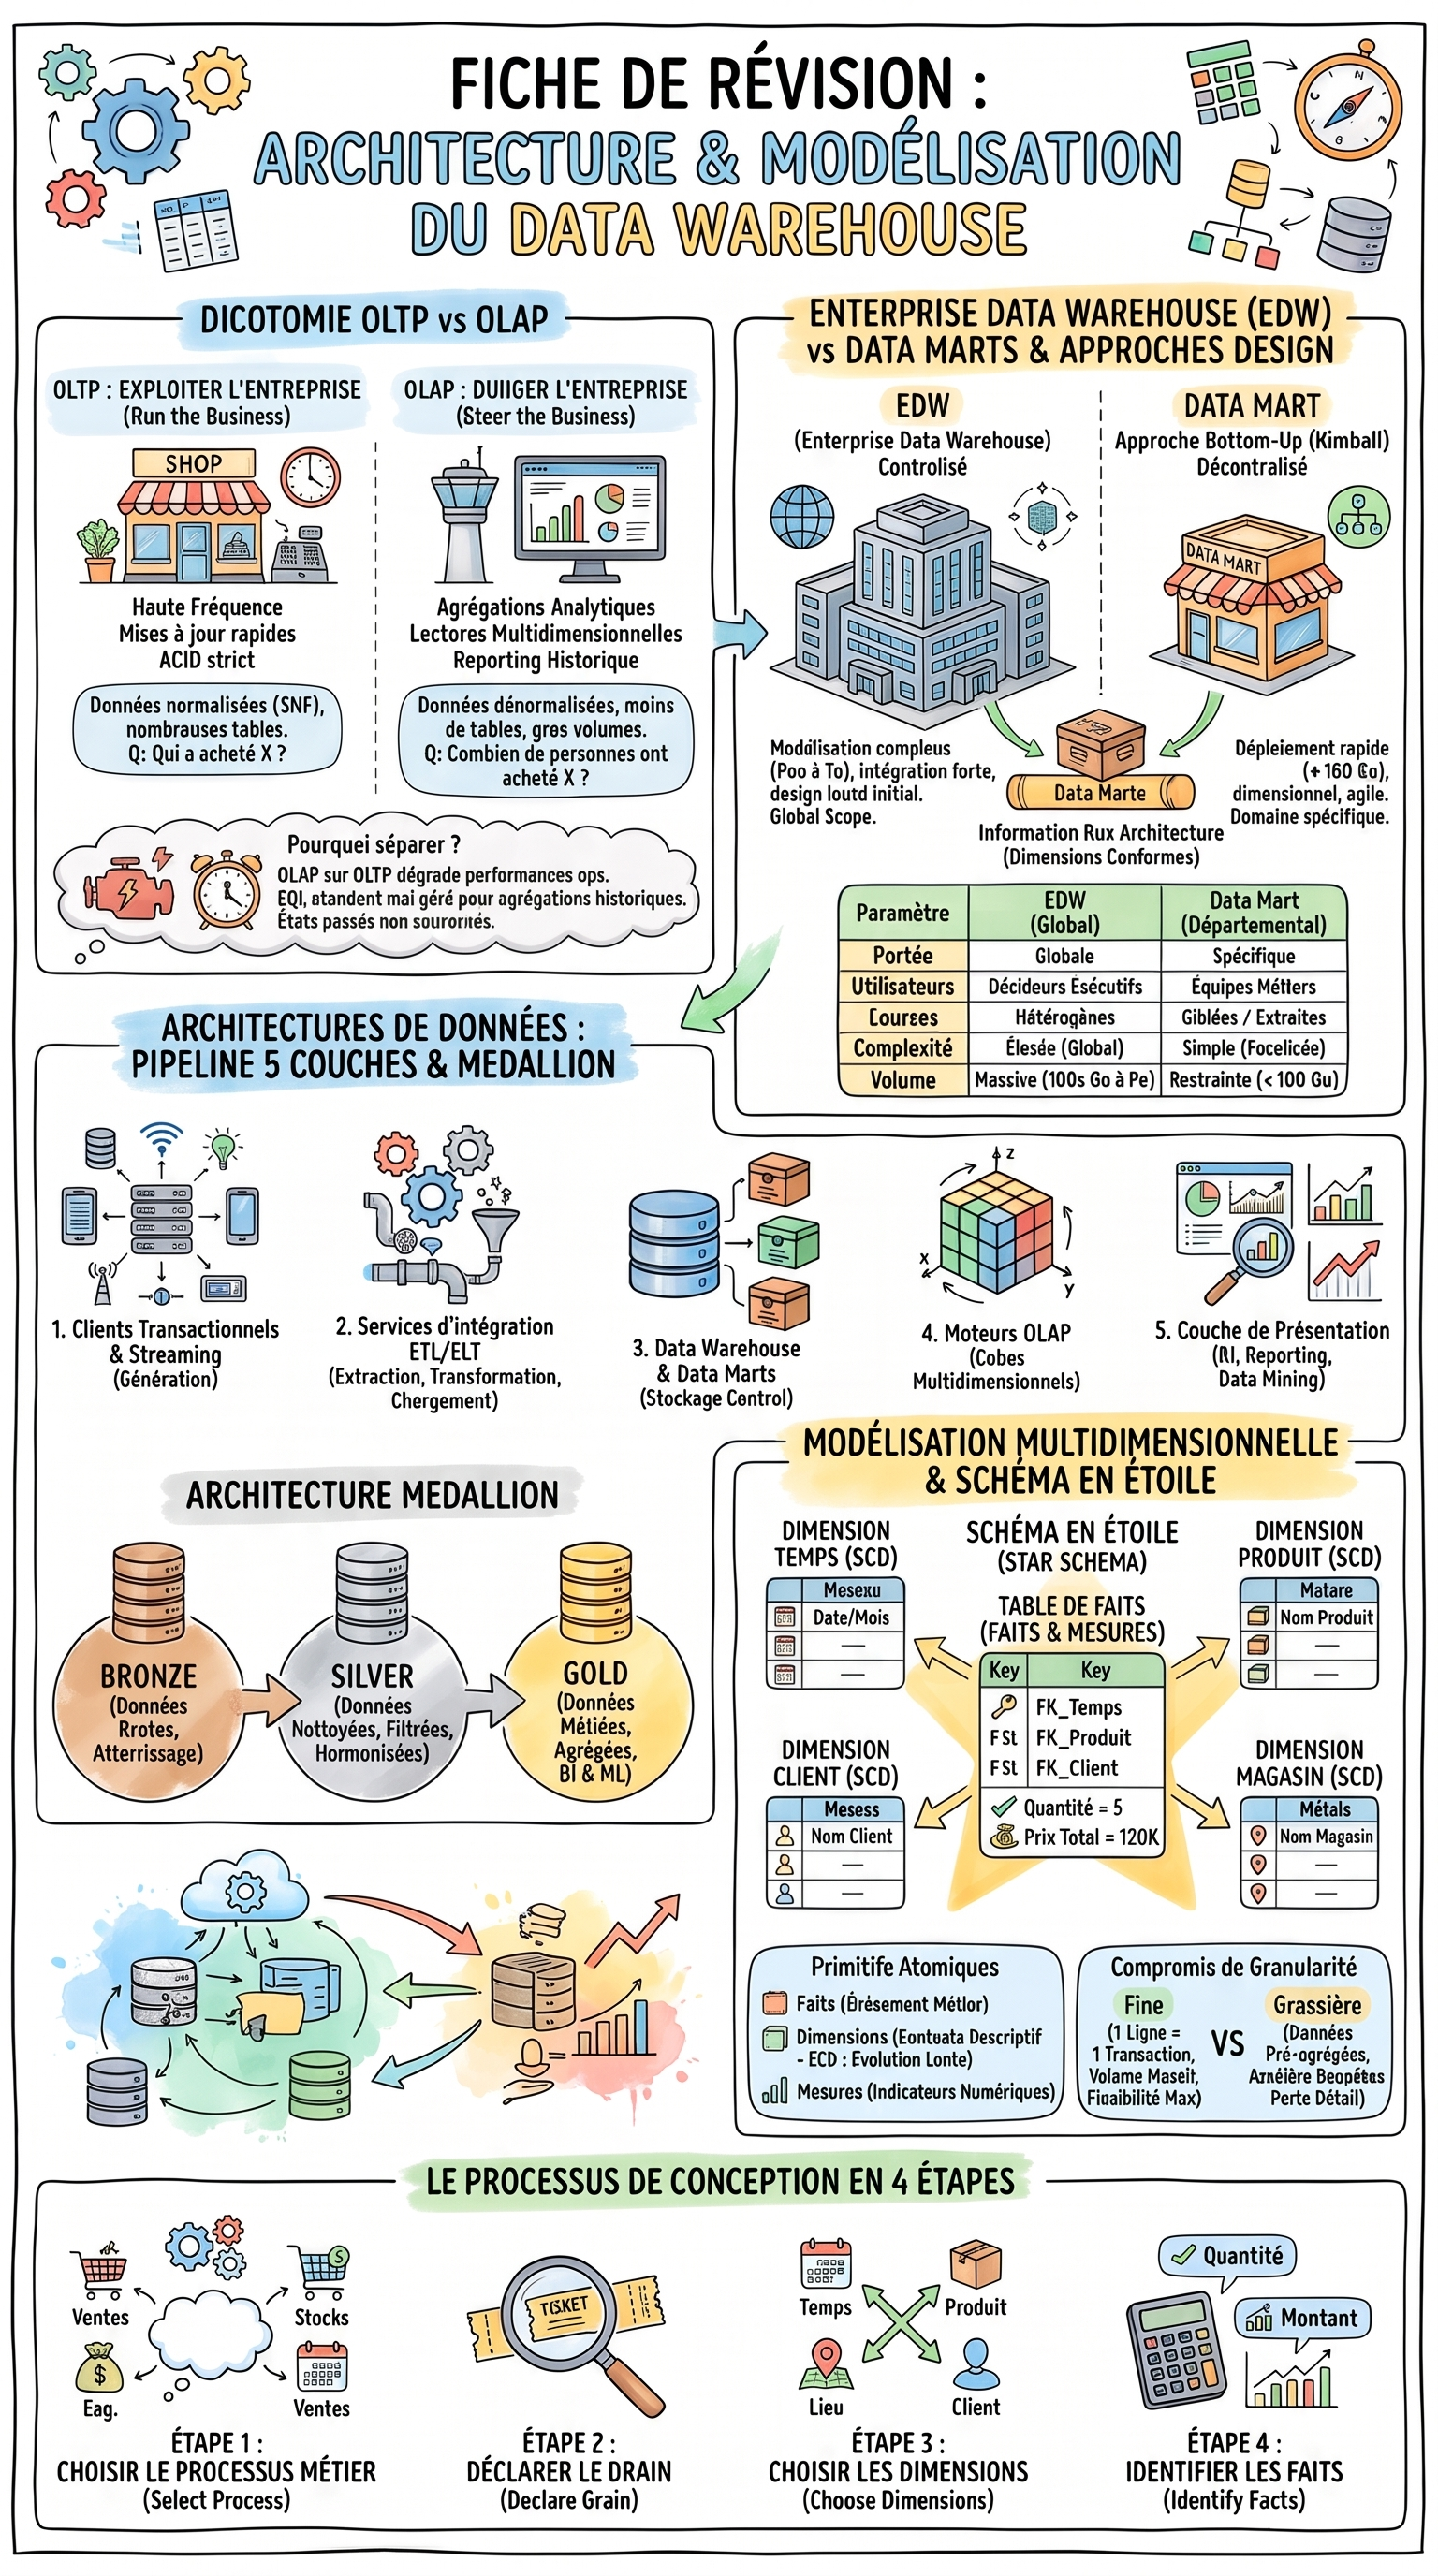
\includegraphics[width=\textwidth, height=0.78\textheight, keepaspectratio]{architecture_data_warehouse.png}
\caption{Fiche de Révision Synthétique : Inmon vs Kimball, EDW vs Data Marts}
\end{figure}

\begin{center}
\renewcommand{\arraystretch}{1.2}
\begin{tabularx}{\textwidth}{p{3.8cm} X X}
\toprule
\textbf{Paramètre} & \textbf{Approche Bill Inmon (Top-Down)} & \textbf{Approche Ralph Kimball (Bottom-Up)} \\
\midrule
\textbf{Vision} & Entrepôt de Données d'Entreprise (EDW) centralisé. & Constellation de Data Marts dimensionnels connectés. \\
\textbf{Structure de l'EDW} & Normalisée en Troisième Forme Normale (3NF). & Schémas en Étoile dénormalisés. \\
\textbf{Déploiement} & Projet global, initialisation lourde et rigoureuse. & Itératif, agile, ROI rapide par département. \\
\textbf{Cohérence globale} & Assurée par le modèle relationnel unifié d'entreprise. & Assurée par les \textbf{Dimensions Conformées} (\textit{Conformed Dimensions}). \\
\bottomrule
\end{tabularx}
\end{center}

\subsection{5. Évolution Lente des Dimensions (SCD : Slowly Changing Dimensions)}
Dans un système décisionnel, les attributs des dimensions évoluent dans le temps (ex: un praticien change de spécialité ou monte en grade ; un patient déménage de Rabat à Casablanca). Kimball formalise trois stratégies canoniques :
\begin{itemize}[label=$\bullet$]
    \item \textbf{SCD Type 1 (Écrasement) :} On met à jour la valeur sans conserver l'historique (\texttt{UPDATE}). Simple, mais fausse l'analyse historique rétrospective.
    \item \textbf{SCD Type 2 (Création d'une nouvelle ligne) :} Méthode de référence. On ajoute une nouvelle ligne dans la table de dimension avec une nouvelle clé surrogate, une date de début de validité, une date de fin, et un drapeau \texttt{est\_actif = TRUE}.
    \item \textbf{SCD Type 3 (Ajout de colonne) :} On ajoute une colonne \texttt{ancienne\_ville} et \texttt{nouvelle\_ville}. Ne permet de conserver qu'un niveau d'historique.
\end{itemize}

% ==============================================================================
% SECTION 4 : GUIDE D'APPRENTISSAGE & MÉTHODOLOGIE D'EXAMEN
% ==============================================================================
\section{Guide d'Apprentissage \& Méthodologie d'Examen}

\subsection{La Démarche Systématique pour Résoudre n'importe quel Sujet}
Lorsque vous découvrez un énoncé d'examen ou un projet professionnel :
\begin{enumerate}
    \item \textbf{Chassez le verbe d'action transactionnel :} Lisez le texte en surlignant l'événement physique qui se produit (vente, consultation, virement bancaire, clic web). Cela vous donne immédiatement le nom de votre \textbf{table de faits}.
    \item \textbf{Fixez sans compromis le grain atomique :} Écrivez en une phrase : \textit{« Le grain représente une occurrence unitaire de [l'événement] »}. Ne commencez jamais par un grain agrégé par mois ou par magasin.
    \item \textbf{Séparez rigoureusement Faits et Attributs :}
    \begin{itemize}
        \item Est-ce mesurable, numérique et cumulable ? $\rightarrow$ C'est une \textbf{mesure} (table de faits).
        \item Est-ce qualitatif, textuel ou utilisé pour filtrer / grouper ? $\rightarrow$ C'est un \textbf{attribut} (dimension).
    \end{itemize}
    \item \textbf{Bannissez les clés naturelles dans la table de faits :} N'utilisez jamais le matricule métier ou le numéro de sécurité sociale comme clé de jointure. Créez systématiquement des clés de substitution (\textit{Surrogate Keys}) de type entier pour garantir la performance des jointures et supporter les dimensions SCD.
    \item \textbf{Formulez des questions croisées pour vos KPI :} Vos questions analytiques doivent toujours croiser au moins une mesure avec au moins deux dimensions distinctes (ex: \textit{Montant total} par \textit{Région} et par \textit{Année}).
\end{enumerate}

\subsection{Les 5 Pièges Fréquents à Éviter Absolument}
\begin{alertbox}{Pièges à Éviter lors des Examens}
\begin{enumerate}
    \item \textbf{Confondre mesure et attribut :}\\
    L'âge du patient peut sembler numérique, mais s'il sert à créer des groupes (0-18, 19-35), c'est un attribut de dimension et non une mesure de la table de faits.
    \item \textbf{Sur-normaliser en flocon inutilement :}\\
    En modélisation décisionnelle, la redondance textuelle dans une dimension est une vertu, pas un défaut ! Ne créez pas de table \texttt{VILLE} séparée de \texttt{REGION} sauf si la modélisation en flocon est expressément exigée.
    \item \textbf{Oublier la dimension Temps :}\\
    Un Data Warehouse est intrinsèquement historisé (\textit{Time-Variant}). Une table de faits sans dimension temporelle est une faute conceptuelle grave.
    \item \textbf{Tenter d'additionner des taux ou des moyennes :}\\
    Les moyennes sont des mesures non-additives. On ne somme jamais des moyennes ; on stocke la somme des valeurs et le nombre d'occurrences pour recalculer la moyenne pondérée globale.
    \item \textbf{Négliger les verrous et la charge OLTP :}\\
    Si une question vous demande pourquoi un système transactionnel ralentit lors de requêtes BI, répondez toujours par la concurrence sur les ressources (CPU, RAM, E/S disque) et les blocages mutuels causés par les verrous de lecture/écriture.
\end{enumerate}
\end{alertbox}

\end{document}
